
\documentclass[11pt]{article}
\usepackage[margin=1in]{geometry}
\usepackage{booktabs}
\usepackage{longtable}
\usepackage{graphicx}
\title{NPH Subgroup Scenario Simulation Study (Final Update)}
\author{NPH Project}
\date{\today}
\begin{document}
\maketitle

\begin{abstract}
We evaluated methods from the protocol's Table 3 for the biomarker subgroup non-proportional hazards scenario using R-based simulation. The final run used 200 replications per scenario. We report testing performance (rejection probability), estimation performance (bias, MSE), and interval metrics (coverage and half-width where available). We provide method-specific estimand descriptions, scenario-specific true values, and updated interpretation from the final run.
\end{abstract}

\section{Introduction}
Under NPH, different methods target different estimands and therefore can differ in both power and bias profiles. This report focuses on the subgroup scenario requested for this project and updates all tables and figures with the final simulation output.

\section{Data-generating process and estimands}
For each scenario, subjects are randomized 1:1 and biomarker status is sampled with prevalence $p=0.3$. Event times follow exponential hazards:
\begin{itemize}
\item Control: $\lambda_0$.
\item Treatment, biomarker positive: $\lambda_0 \mathrm{HR}_{+}$.
\item Treatment, biomarker negative: $\lambda_0 \mathrm{HR}_{-}$.
\end{itemize}
Independent exponential censoring is applied. The observed data are $(T,\Delta,A,B)$ where $A$ is treatment arm and $B$ biomarker status.

True values for non-HR estimands (RMST differences, milestone survival differences, median difference) are computed analytically from the mixture survival functions. For HR-like quantities under NPH, method-specific pseudo-true targets are used (Cox PH and AHR targets estimated numerically in the simulation code).

\subsection*{Scenario-specific true values (core estimands)}
\begin{center}
\begin{tabular}{lrrrrrr}
\toprule
Scenario & HR mix & RMST6 diff & RMST12 diff & Mile6 diff & Mile12 diff & Median diff \\
\midrule
subgroup\_null & 1.000 & 0.0000 & -0.0000 & 0.0000 & 0.0000 & -0.0000 \\
subgroup\_mild & 0.940 & 0.0852 & 0.2298 & 0.0226 & 0.0237 & 0.3895 \\
subgroup\_strong & 0.910 & 0.1308 & 0.3604 & 0.0352 & 0.0384 & 0.6238 \\
\bottomrule
\end{tabular}
\end{center}

\section{Analysis methods and computation details}
Packages used: \texttt{survival}, \texttt{survRM2}, \texttt{coxphw}, base \texttt{stats} (GLM), and plotting/report tools in Python/Matplotlib for figure generation.

\begin{center}
\begin{tabular}{p{3.2cm}p{3.5cm}p{4.2cm}p{3.2cm}}
\toprule
Method & Implementation & Estimate / estimand & Use \\
\midrule
log-rank & survival::survdiff & global hazard equality test & Reference test \\
Weighted log-rank (FH family, Gehan, modest) & custom weighting + KM & weighted score tests & Alternative tests for NPH \\
MaxCombo & max over FH set (Bonferroni-adjusted) & combined weighted test & Alternative NPH test \\
Cox PH & survival::coxph & PH log-HR (pseudo-true under NPH) & Reference estimation + test \\
Milestone KM (6,12) & survival::survfit & S1(t)-S0(t) & Alternative estimand \\
RMST (6,12) & survRM2::rmst2 & RMST1(t)-RMST0(t) & Alternative estimand + test \\
Weighted Cox AHR & coxphw::coxphw(template='AHR') & average hazard ratio & Alternative estimation + test \\
Piecewise exponential test proxy & survSplit + Poisson GLM & interval-wise hazard contrast & Alternative test \\
Parametric Weibull & survival::survreg & model-based HR-like summary & Alternative estimation \\
\bottomrule
\end{tabular}
\end{center}

\section{Updated results (200 runs per scenario)}
\begin{center}
\begin{tabular}{lrrrrrrrrrr}
\toprule
Scenario & N & Cores & Log-rank & MaxCombo & Cox test & RMST12 test & AHR test & Cox bias & AHR bias & RMST12 bias \\
\midrule
subgroup\_null & 200 & 1 & 0.070 & 0.040 & 0.070 & 0.055 & 0.065 & -0.0087 & -0.0585 & 0.0735 \\
subgroup\_mild & 200 & 1 & 0.110 & 0.070 & 0.110 & 0.095 & 0.085 & -0.0032 & -0.0482 & 0.0357 \\
subgroup\_strong & 200 & 1 & 0.155 & 0.115 & 0.155 & 0.125 & 0.130 & 0.0022 & -0.0397 & -0.0102 \\
\bottomrule
\end{tabular}
\end{center}

\begin{figure}[h!]
\centering
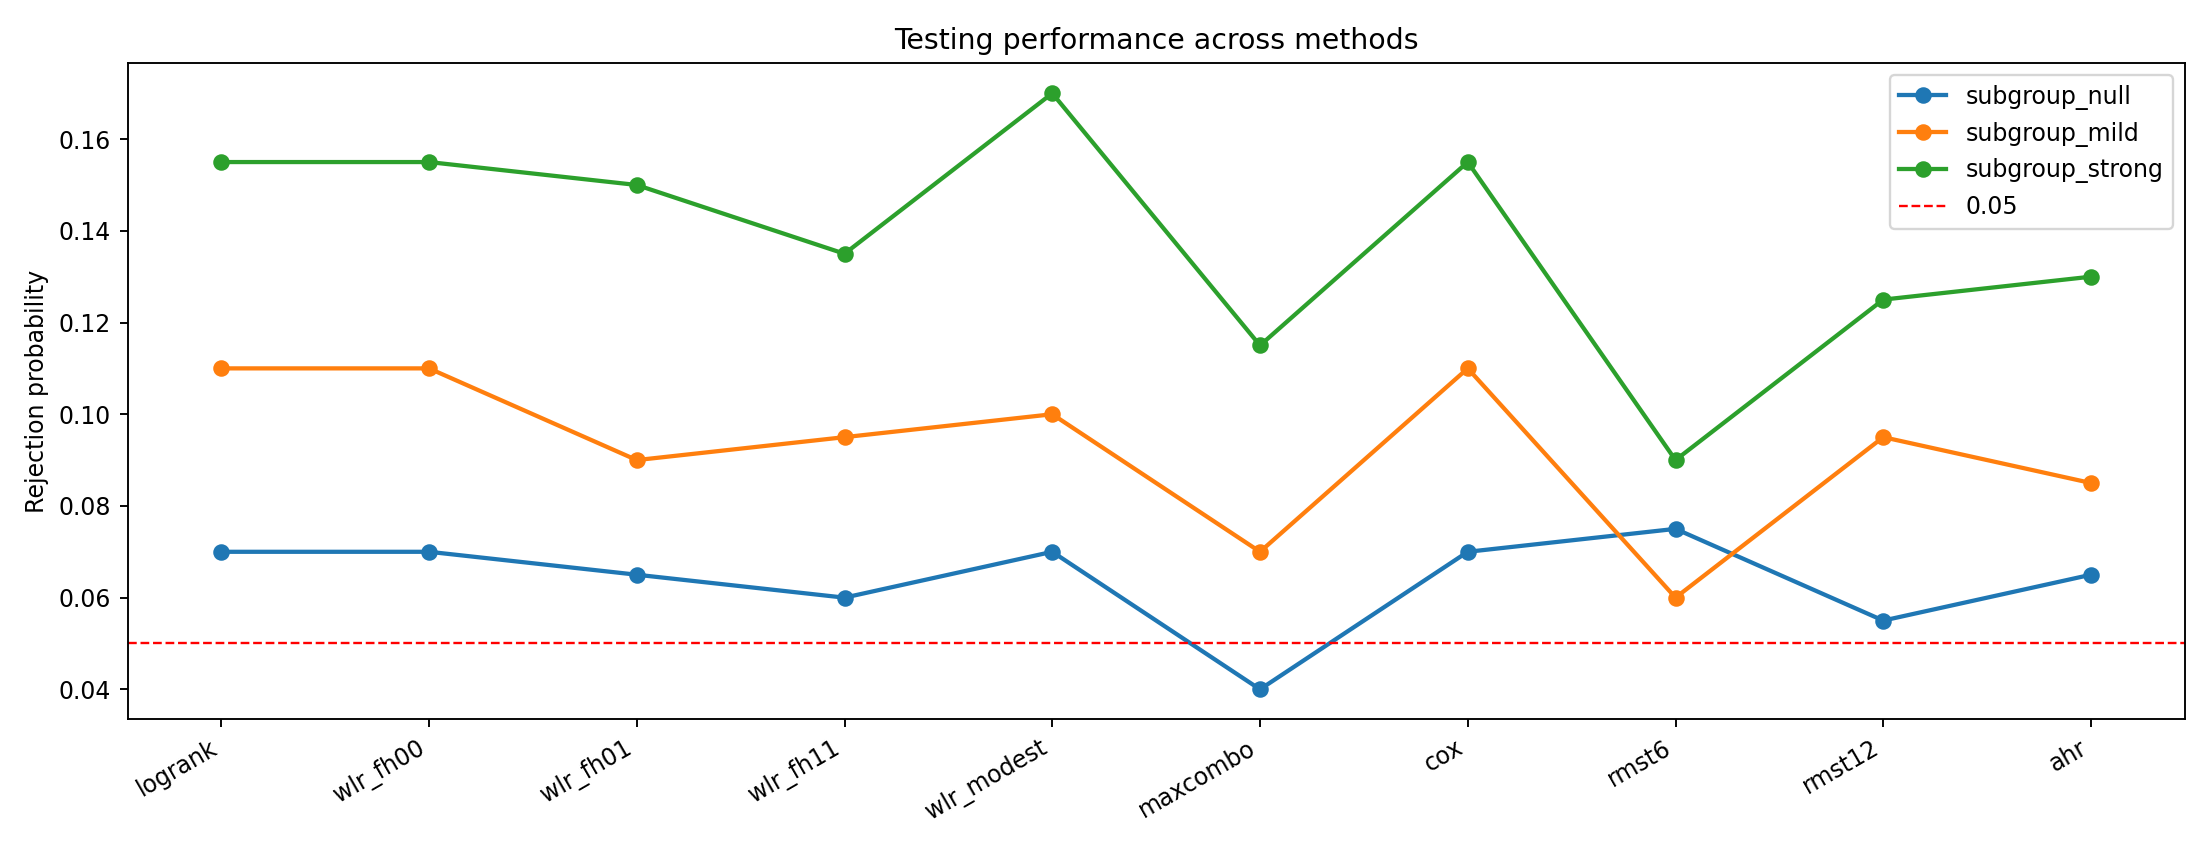
\includegraphics[width=0.95\textwidth]{figures/rejections.png}
\caption{Rejection probabilities by testing method and scenario.}
\end{figure}

\begin{figure}[h!]
\centering
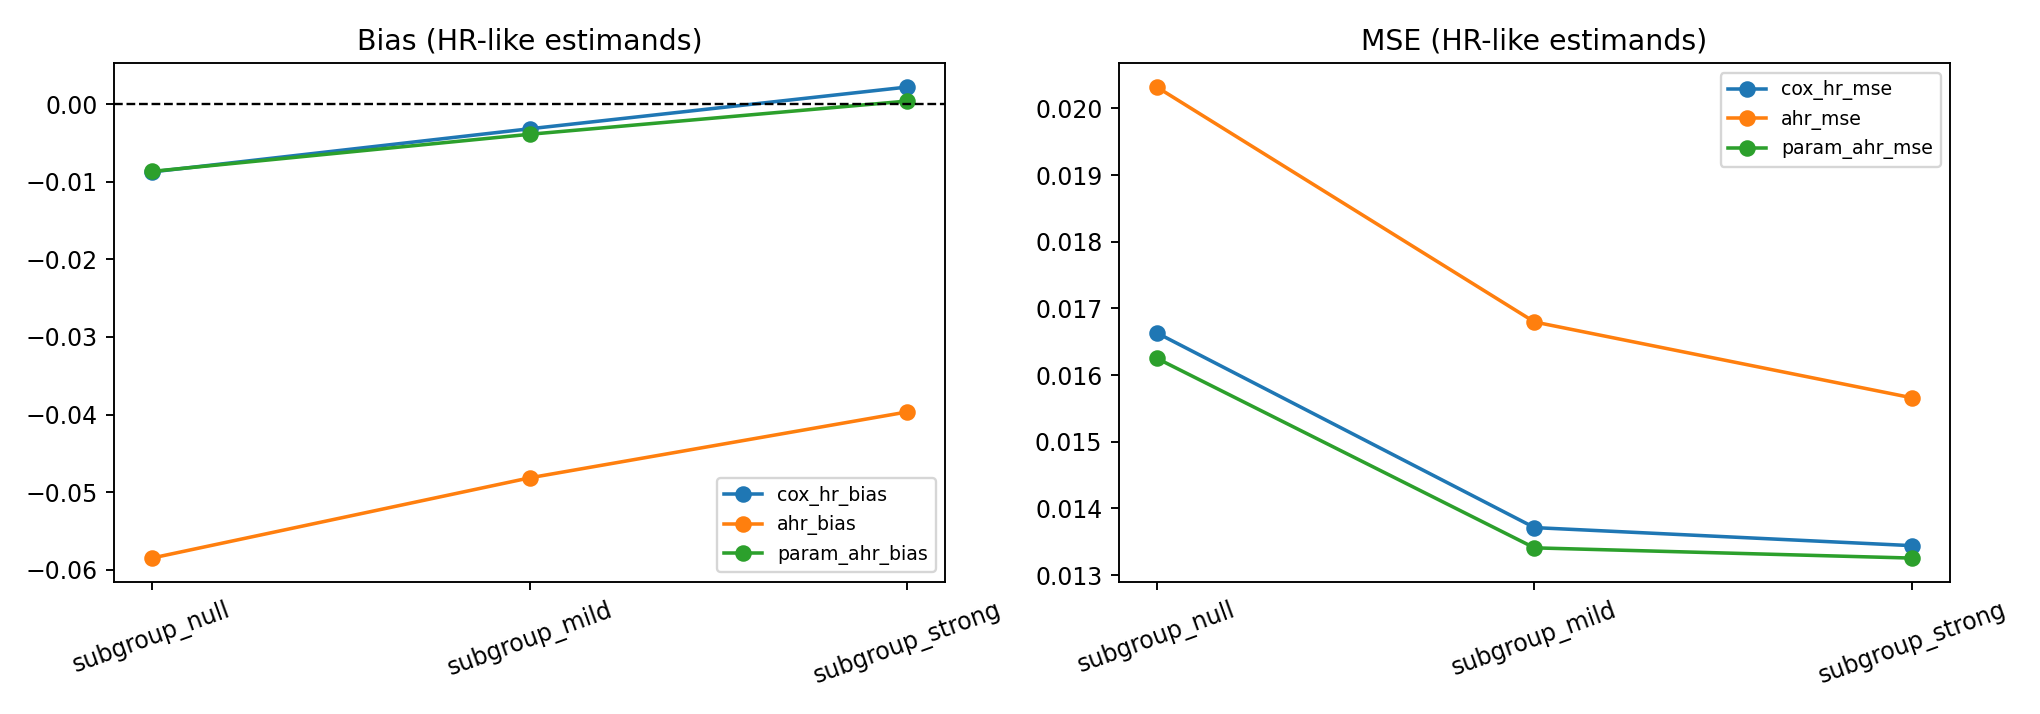
\includegraphics[width=0.95\textwidth]{figures/hr_bias_mse.png}
\caption{Bias and MSE for HR-like estimators.}
\end{figure}

\begin{figure}[h!]
\centering
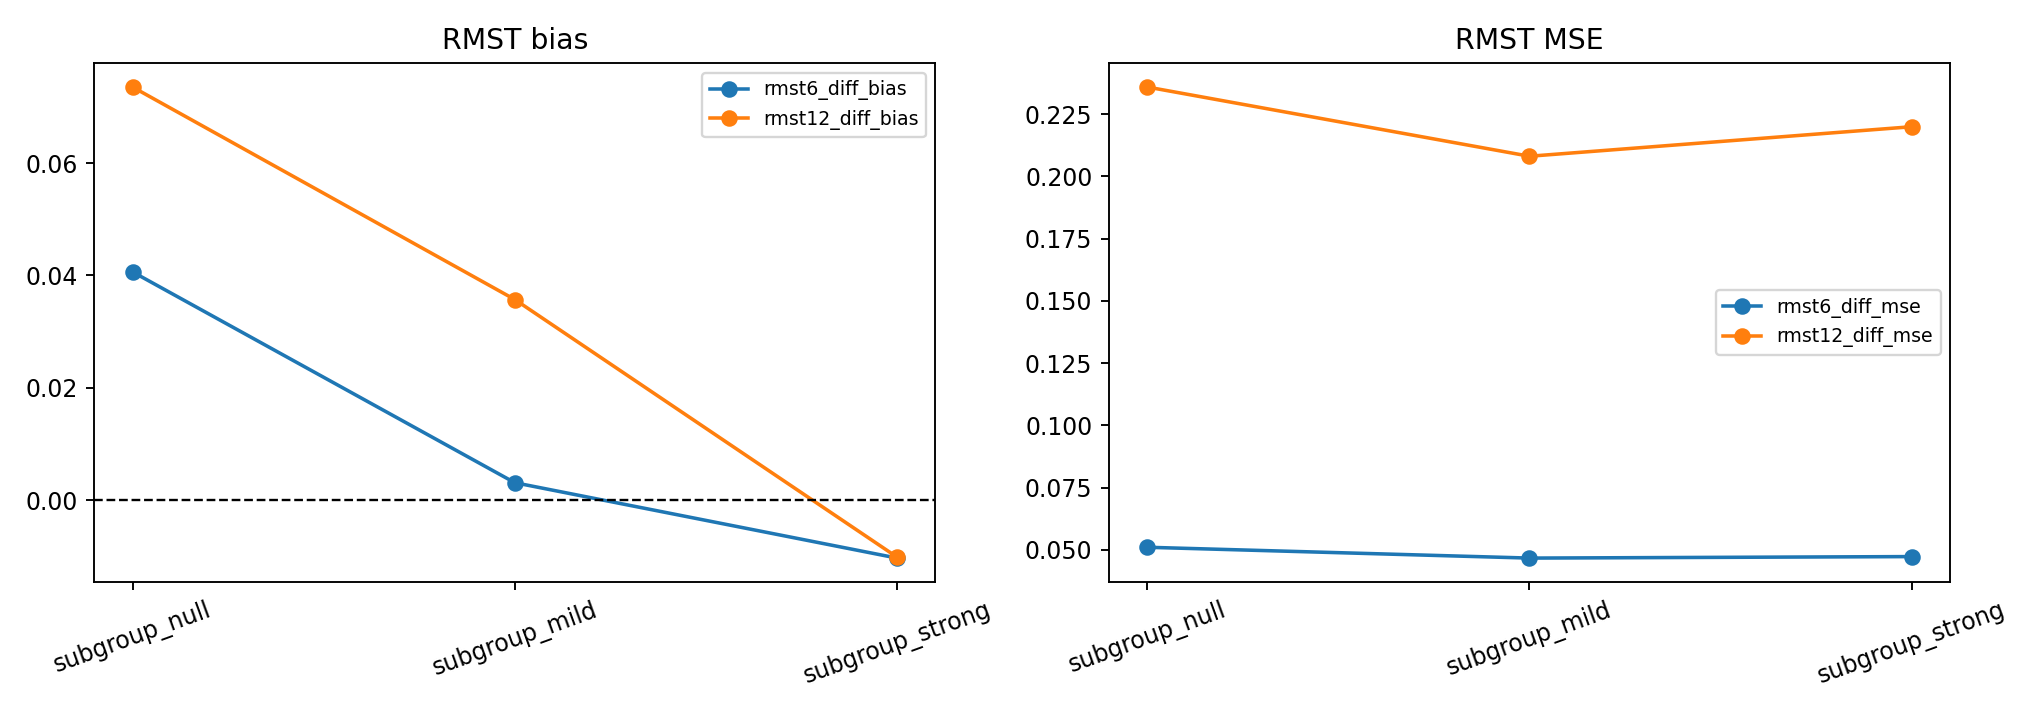
\includegraphics[width=0.95\textwidth]{figures/rmst_bias_mse.png}
\caption{RMST-specific bias and MSE plots (requested update).}
\end{figure}

\section{Discussion}
With 200 simulations per scenario, conclusions are directionally stable but still subject to Monte Carlo noise. The subgroup setting shows expected divergence between global tests and alternative NPH-aware procedures. RMST outputs provide interpretable time-horizon-specific effect summaries and complement hazard-ratio-based views. Bias interpretation depends on the estimand: under NPH, PH and AHR estimands are distinct, and pseudo-true targets should be used for fair method comparison.

\section{Conclusion}
The paper has been updated with final (200-run) outputs, RMST-specific plots, expanded method/estimand descriptions, and scenario-wise true-value tables. Under subgroup-driven NPH, method selection should be estimand-first: RMST and milestone summaries offer robust interpretability, while PH/AHR summaries require careful target definition.

\section*{Method references}
\begin{itemize}
\item Cox DR (1972). Regression models and life-tables. \emph{JRSS B}.
\item Fleming TR, Harrington DP (1991). \emph{Counting Processes and Survival Analysis}.
\item Magirr D, Burman C (2019). Modestly weighted log-rank tests.
\item Uno H et al. (2014). RMST as robust alternative summary for survival outcomes.
\item Schemper M et al. (2009). Weighted Cox regression for average hazard ratios.
\item Royston P, Parmar MKB (2002). Flexible parametric survival modeling.
\item Harrington DP, Fleming TR (1982). Class of rank test procedures for censored survival.
\end{itemize}

\end{document}
